\chapter{Web extraction / TODO}

Since we know the central concepts related to a webpage and its structure, we can talk about the Web extraction (WE) problem in detail. In this chapter, we will discuss modern techniques used in this area such as crawlers, wrappers and also list the complementary problems as named entity recognition and region extraction. At the end of the chapter, we will discuss related work to the thesis.\\

\textit{Web extraction} (also Web Scraping, Web harvesting) is the extraction of structured information from a webpage presented as an HTML, i.e. semi-structured text. It is important to highlight that by saying that we \textit{extract} the information from a webpage, we assume the information is located on the page and readable.


\section{Information Extraction / TODO}

The goal of Information Extraction (IE) is an automatic identification and extracting structured information from unstructured or semi-structured documents. Most of the time, in IT one processes human language. The information needed to be extracted must be explicitly specified. IE is a non-trivial task due to the complexity of natural language, and even for a limited domain implies a lot of work.\\

IE consists of several sub-tasks \cite{InfExtr}:

\begin{enumerate}
    \item \textit{Named Entity Recognition} (NER) refers to the problem of the identification and classification of predefined types of named entities, such as organizations, persons, place names, time, etc.
    \item \textit{Co-reference Resolution} (CO) requires the identification of co-referring mentions of the same entity.
    \item \textit{Relation Extraction} (RE) detects and classifies predefined relationships between identified entities.
    \item \textit{Event Extraction} (EE) refers to an identifying event in text and deriving structured information like who did what to whom, when, where, through what methods, and why. Don't confuse this sub-task of IE with the Event Extraction in the thesis, where we consider social events rather that relationships between entities in the natural language text. 
\end{enumerate}

These four sub-tasks can be considered as four well-known problems: NER refers to a segmentation and classification, RE is the association and EE is a clustering \cite{ManLect}.\\

\section{Web extraction methods}

% READ WIKI https://en.wikipedia.org/wiki/Web_scraping#Techniques\\ \cite{WikiScrap}

WE can be seen as a particular case of IE where the entities are extracted not from a plain natural language text, but rather from a semi-structured HTML page. WE implies several additional sub-tasks specifically related to a webpage structure. For example, Region Extraction (RE) helps to filter web elements to focus only on relevant information. Also, since WE works with an HTML, it must entail its structure and process the tree rather than plain text. \\

World Wide Web Consortium (W3C) is an international standard organization tries to get all the players on the Web implement the same set of core principles and components. That is why all websites use relatively the same stack of technologies, and browsers seek to follow all changes and support major updates in popular web tools.\\

Despite the fact, web developers use the same tools, HTML pages of different websites most of the time are completely different. Every site is following its design and structure, presenting the information in a different way for the particular audience of the website. That means if one method of WE works well on a specific site, it won't probably work for other websites with the same information. For that reason, WE needs to solve the problem of heterogeneity of the websites, which is the most difficult part of WE field.

\subsection{XPath and CSS}

One of the popular methods of WE from a webpage is using XPath and CSS selectors for identifying and extracting the information. The algorithm is quite simple: you look to an HTML code, find those blocks which you need to extract and compose correct XPath or CSS selectors for these web elements. After that, you can obtain the information on any webpage where such path in a DOM tree exists.  This method is the most appropriate and fast if you have one website with a big number of static pages with identical structure and design. \\

In our thesis, we use this approach as one of the steps of dataset collecting. We use Scrapy Python framework \cite{Scrapy} for identifying semantic Metadata tags and crawling the text corresponding to each tag. See example of code with Scrapy on the listing \ref{list:scrapy}.\\

\begin{lstlisting}[language=Python, caption={Example of meta tag text scrapping with Scrapy Python framework}, label={list:scrapy}, captionpos=b]
from scrapy.selector import Selector
import urllib.request as request

def get_item_types(url):
    item_types = []
    page = request.urlopen(url)
    if page.code == 200:
        html_body = page.read()
        selector = Selector(text=html_body, type="html")
        elements = selector.xpath('.//*[@itemscope]')
        for item in elements:
            item_type_text = item.xpath('@itemtype').extract()
            item_types.append(item_type_text)
    return item_types 
\end{lstlisting}

The code is self-explainable, but let's briefly discuss the main steps. Firstly, you open the webpage with urllib, that's where we send an HTTP request. If the status code is 200, meaning the positive answer from a server, we read the page. We create Scrapy Selector, and in this case, we use XPath locator. We are identifying all elements which have 'itemscope' attribute meaning we want to extract all elements which tagged with any semantic label. Then in a loop we collect all types of these semantic tag names, for example 'http://schema.org/Person', 'http://schema.org/Movie', 'http://schema.org/Event', 'http://schema.org/Place', etc. The name of the Metadata tag takes the form of URL for simplicity. \\

Obviously, the problem with this approach is no scalability, because the path in a DOM for different websites would be different. \\

\subsection{Wrappers}

\textit{Wrapper} is a general name for a program for data extraction from a webpage. In the practical application such programs are also called \textit{web crawlers} (or web spiders, web scrapers). Typically, wrappers are implemented manually by a programmer, and she needs to create a new specified wrapper for every document which has to be processed. The output of a wrapper is a structured information in some machine readable format. \\

\noindent Wrappers can be divided into three segments depending on the level of automation:
\begin{itemize}
    \item Manual wrapper: the user observers a webpage, its source code and writes down a program code to extract data (for example, using the XPath and CSS).
    \item Wrapper induction: supervised learning where extraction rules are learned from a manually labeled data records \cite{Hsu}, \cite{BotUp}, \cite{Stalker}, \cite{Wien}, \cite{Rapier}\cite{SRV}\cite{Vide}. The inductive learning process is the generalization of wrappers that are obtained from human labeled documents. 
    \item Automatic wrapper induction: unsupervised learning with the use of tree matching algorithms to find repetitive patterns on single or multiple pages \cite{Qiu}, \cite{Dalvi}, \cite{Diadem}, \cite{Roadrunner}, \cite{LiuMinData}, \cite{Urest}. Automatic wrapper induction is possible because a lot of web objects follow fixed templates.
\end{itemize}

Typical usage of the wrapper as follows: a user defines set of desired attributes and indicates associated fragments of the example page. Then the program learns a wrapper for the current website. After it is done, the program uses the learned wrapper to extract new information from the same source automatically. Therefore, every step of this process may be automated to some degree. \\

Wrappers usually work well on template-based web pages, for example, a list of addresses, product catalogs, and telephone directories. There is a problem with more unstructured page with custom design, but this kind of webpages are common on the web.

\section{Adaptive Information Extraction}

Adaptive information extraction methods can handle less structured webpages. There are three main approaches:

\begin{enumerate}
    \item First approach considers extraction task as a Classification problem which has the learning and prediction stages. For this method, one needs to have a dataset with labeled entities which needed to be extracted. 
    \item In the Sequential Labeling approach, a webpage is viewed as a sequence of words (tokens). This method can model the dependencies between target entities on the page while the classification task considering each entity independently.
    \item Visual Information Extraction relies on rendering a webpage in a browser. This approach helps in extracting objects from complex web pages that may exhibit a visual pattern, but a lack of patterns in the HTML code.
\end{enumerate}

The current thesis falls into the Classification-based approach with one exception: we generate the training dataset automatically and don't imply human labeling procedure. Also, we use visual features from rendered webpage, means use ideas from Visual Information Extraction approach.\\  

More extensive surveys on different methods and works in Web Extraction field can be found in \cite{WebExtraSurveyFerrara},  \cite{Trends}, \cite{WebDataSurvey}.

% \cite{AutoWrapLect}
% http://www.isi.edu/integration/courses/csci548_2010/slides/Wrapper_Generation.pdf
% COPY%


% [LIU11] [Bing Liu. Web Data Mining: Exploring Hyperlinks, Contents, and Usage Data. Springer-Verlag New York, Inc., Secaucus, NJ, USA, 2011.] \cite{WebDataMining}

% [Robert Baumgartner, Thomas Eiter, Georg Gottlob, Marcus Herzog, and Christoph Koch. Information Extraction for the Semantic Web. In Nor- bert Eisinger and Jan Maauszy«ski, editors, Reasoning Web, number 3564 in Lecture Notes in Computer Science, pages 275 289. Springer Berlin Hei- delberg, 2005. DOI: 10.1007/11526988\_8.] \cite{InfExtrSemWeb}



\section{Related problems / TODO}

\subsection{Information retrieval / TODO}

Information Extraction is closely related to Information Retrieval (IR). 
The task of IR is to select from a collection of textual documents a subset which are relevant to a particular query, based on key-word search and possibly augmented by the use of a thesaurus \cite{InfExtr}. A simple example of IR application is a search engine websites. You set the query and as an output of IR algorithm you have a list of relevant documents, ranked in descending order. In general case, there is not extracted answer from a corpus of documents, only the documents where the answer might be. To extract the facts or meaningful structured information from a document one needs to understand the semantic of the text on a webpage. And that's the main goal of IE.

IE task considered to be more difficult than IR. However, IR and IE techniques are complementary and may be combined in different ways. IE often uses the IR as a filtering step, because usually, the corpus of texts where the IE is extracting the information is very large. IR often uses IE for the feature extraction.\\

\begin{figure}[h]
\begin{center}
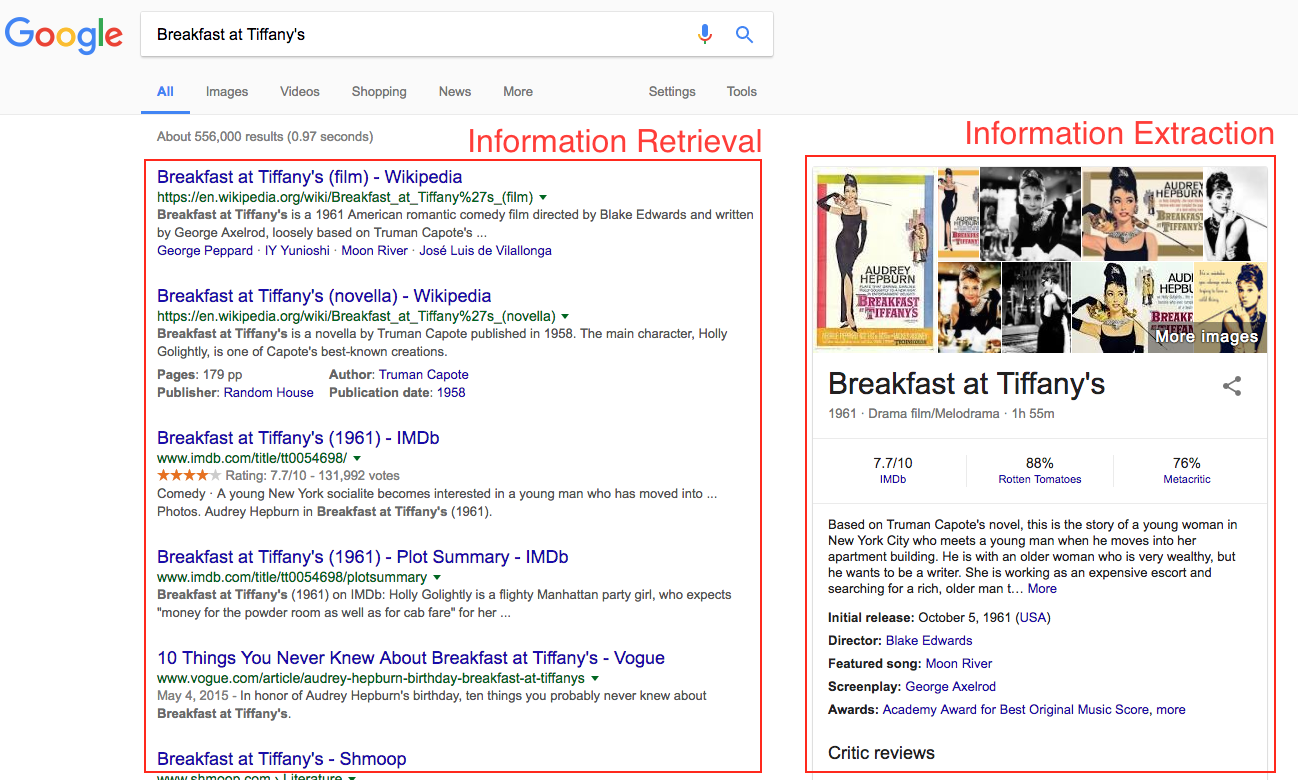
\includegraphics[width=1.0\textwidth]{figures03/retrieval_extraction}
\caption{The difference between Information Extraction and Information Retrieval}
\label{fig:architecture}
\end{center}
\end{figure}


\subsection{Named Entity Recognition}
\textit{Named Entity Recognition (NER)} is the task of extracting entities, such as proper name (person, location and organization), time (date and time), and numerical values (currency and percentage), from the source text, and mapping them into predefined categories, such as person, organization, location name or “none-of-the-above” \cite{MaxEntropy}. The two main components of NER are \textit{to find} the entity and then \textit{classify} this entity. \\

NER is a main sub-task of IE.  

[7 A. Borthwick. A Maximum Entropy Approach to Named Entity Recognition. Phd thesis, New York University, 1999.] \\
% [lectures source https://web.stanford.edu/class/cs124/lec/Information_Extraction_and_Named_Entity_Recognition.pdf]

There three main techniques for NER (and IE): 
\te
Hand-written regular expressions\\
Using classifiers
• Generative: Naïve Bayes
• Discriminative: Maxent models\\
Sequence models
• HMMs
• CMMs/MEMMs\\


\subsection{Region extraction / TODO}

% Article http://80.ieeexplore.ieee.org.dialog.cvut.cz/stamp/stamp.jsp?arnumber=6231632&tag=1
\cite{RegExtrSurvey}

Web documents are getting more and more sophisticated,
which complicates the task of information extraction. This
has motivated using region extractors so that information
extractors can focus only on data records or data regions\\

All of the region extractors work on semistructured
documents that are formatted in HTML and rely on
their DOM t\\
Repetetive structure\\
The majority of region extractors are unsupervised
and usually rely on the following algorithms: Tree
matching, string matching, and clustering.\\

 The difference
between information extractors and region extractors is that
the former focus on extracting and structuring data records
and their attributes, whereas the latter focus on identifying
the HTML fragments that contain this information. Y \\

State of the art Region extraction\\
3.3 MDR: Mining Data Records\\
Mining Data Records [100], or MDR for short, is intended to
extract data records. It builds on the hypothesis that a data
region contains a repetitive structure in a document, that
each repetitive structure inside a data region is a data
record, and that data records are usually rendered inside
tables and forms.\\
\cite{LiuMinData} [100] B. Liu, R.L. Grossman, and Y. Zhai, “Mining Web Pages for Data
Records,” IEEE Intelligent Systems, vol. 19, no. 6, pp. 49-55, Nov./
Dec. 2004.\\

y Embley et al. [53] \\
The proposal by Embley et al. [53] is intended to extract the
data records from the largest data region in a web document.
It builds on the hypothesis that there is a unique data region,
which is the largest region in the web document, that this
region contains multiple data records, that some tags are
more likely to be data record separators based on their
type and their occurrences, and that counting on an
ontology helps identify data records.\\

\cite{Embley} [53]] D.W. Embley, Y.S. Jiang, and Y.-K. Ng, “Record-Boundary
Discovery in Web Documents,” Proc. ACM SIGMOD Int’l Conf.
Management of Data, pp. 467-478, 1999.\\

Yi et al.\\
[175], Wang and Lochovsky [163], and Kang and Choi [84]
have confirmed experimentally that using region extractors
has a positive impact on both efficiency and effectiveness; it
is not surprising then that some recent proposals for
information extraction incorporate a built-in region extractor
[98], [99], [143], [164], [178]. Beyond information
extraction, region extractors have also proven to be useful
for information retrieval [176], focused web crawling [25],
[32], topic distillation [31], adaptive content delivery [82],
mashups [152], and metasearch engines [113].\\

\cite{Noisy}[175] L. Yi, B. Liu, and X. Li, “Eliminating Noisy Information in Web
Pages for Data Mining,” Proc. ACM SIGKDD Ninth Int’l Conf.
Knowledge Discovery and Data Mining (KDD), pp. 296-305, 2003. \\

\cite{Wang}[163] Wang and F.H. Lochovsky, “Data-Rich Section Extraction from
HTML Pages,” Proc. Third Int’l Conf. Web Information Systems Eng.
(WISE), pp. 313-322, 2002\\

\cite{Kang} [84] J. Kang and J. Choi, “Recognising Informative Web Page Blocks
Using Visual Segmentation for Efficient Information Extraction,”
J. Universal Computer Science, vol. 14, no. 11, pp. 1893-1910, 2008.\\

OMINI [23] \\
OMINI [23] is intended to learn rules to extract data records
from web documents that contain multiple data records in a
unique data region. It builds on the hypothesis that there is
a unique data region in the web document, that this region
corresponds to the subtree with the largest number of
children, and that some tags are more likely to be data
record separators based on their occurrences and type.
OMINI is a constituent part of the information extraction
toolkit called XWRAP Elite [71]\\

[23] ] D. Buttler, L. Liu, and C. Pu, “A Fully Automated Object
Extraction System for the World Wide Web,” Proc. Int’l Conf.
Distributed Computing Systems (ICDCS), pp. 361-370, 2001\\

% U-REST: Unsupervised Record Extraction
% SysTem
% Unsupervised Record Extraction SysTem [141], or UREST
% for short, is intended to extract data records. It builds
% on the hypothesis that data records in a document belong to
% a unique data region, have similar DOM trees, have similar
% structure, and have small separators, if any.\\

%  [141] Y.K. Shen and D.R. Karger, “U-REST: An Unsupervised Record
% Extraction System,” Proc. Int’l Conf. World Wide Web (WWW),
% pp. 1347-1348, 2007.\\

VIPS: Vision-Based Page Segmentation
VIsion-based Page Segmentation [24], or VIPS for short, is
intended to find all of the regions of which a document is
composed. It builds on the hypothesis that web designers
provide visual cues that help people recognize the different
regions of which a document is composed, e.g., horizontal
or vertical rules, boxes, colored panels, special fonts, or
background images. \\
\cite{Vips} [24] D. Cai, S. Yu, J.-R. Wen, and W.-Y. Ma, “Extracting Content
Structure for Web Pages Based on Visual Representation,” Proc.
Fifth Asia Pacific Web Conf. (APWeb), pp. 406-417, 2003.\\

Article of this guy: A Densitometric Approach to Web Page Segmentation\\

\cite{Kohlschutter} [A Densitometric Approach to Web Page Segmentation] we de- scribe a new approach to segment HTML pages, building on methods from Quantitative Linguistics and strategies bor- rowed from the area of Computer Vision. We utilize the notion of text-density as a measure to identify the individ- ual text segments of a web page, reducing the problem to solving a 1D-partitioning task.\\



\section{Recall and Precision / TODO}

Named entity extraction\\
Precision, Recall, and the
F measure;\\
p.17 of presentation
% https://web.stanford.edu/class/cs124/lec/Information_Extraction_and_Named_Entity_Recognition.pdf
\cite{MoensBook} chapter 8 [source http://www.cs.sjtu.edu.cn/~li-fang/IEchapter8.pdf]

\section{Web extraction as a service}

Since the task of automatic web extraction is sought after, there are many commercial applications written for solving this task. There are both desktop and web, free and paid applications with different functionality for the extraction of specific entities. Let's consider those services which provide this functionality as an API.\\

Such applications usually offer their services on a paid basis (per number of requests) and allow to use it by any other application through HTTP requests. These APIs normally extract only specific list of structured information. So it might be an API only for reviews or for example, only for product description in the online store. Below you will find popular web services and their main features.\\

\noindent \textbf{Diffbot's Automatic APIs} automatically extracts the content from supported page types: articles, discussions, images, video and products. It combines a variety of comprehensive techniques such as computer vision and machine learning. It accurately extracts clean and structured data from a webpage in JSON format without and prepossessing steps and training. One particular thing about Diffbot is that it can parse text in different languages because of extracting visual features, not only text content. \cite{Diffbot} [https://www.diffbot.com/]\\

\noindent\textbf{ParseHub} parses the structured data after one example given by the user. It has an interface where the user needs to select several elements which she wants to parse, compose the rule using the visual builder and then run this scenario for the entire page. ParseHub automatically explores all elements which the user meant and parse it to JSON format. After that, this script is available as an API.    
\cite{ParseHub} [https://www.parsehub.com/]\\

\noindent\textbf{Apifier} is similar to Diffbot extracts structured information for specific topics as a product, social networks details, booking hotel websites and search engine. It presents the data in JSON format. 
\cite{Apifier} [source: https://www.apifier.com/] \\

\noindent\textit{Import.io} TODO Read about it
\cite{Importio}[source https://www.import.io/]

\noindent \textit{Mozenda} \cite{Mozenda}

\noindent \textbf{IBM Watson} has an Alchemy Language (part of Natural Language Understanding API) component which analyzes the data on a webpage, extracts specific entities such as people, places, and organizations with NLP methods and answer questions about these entities and its relations. IBM Watson is a huge project and includes a lot of different components related to natural language understanding, speech, and visual recognition.     
\cite{IBMAlchemy} [source https://www.ibm.com/watson/developercloud/alchemy-language.html] \\

\noindent\textbf{Other services}. There are dozens of web services which offer article content extraction, especially the name and description. Also there several interesting services which extract entities from an unstructured plain text: Ambiverse Natural Language Understanding \cite{Ambiverse}, Google Cloud Natural Language \cite{GoogNLP}. Entities are identified by types such as person, location, organization, or product.\\
% [source https://www.ambiverse.com/]\\
% [source https://www.programmableweb.com/category/extraction/api]\\
% [source https://cloud.google.com/natural-language/docs/reference/rest/]\\


\section{Related works / TODO}

\cite{RegExtrSurvey} [source: A Survey on Region Extractors from Web Documents Hassan A. Sleiman and Rafael Corchuelo http://80.ieeexplore.ieee.org.dialog.cvut.cz/stamp/stamp.jsp?arnumber=6231632&tag=1] \\

\cite{GoogEvent} [source Learning to Extract Local Events from the Web http://static.googleusercontent.com/media/research.google.com/ru//pubs/archive/43796.pdf] \\

Petrovski et al. use Schema.org annotations
for products to learn regular expressions that help identify
product attributes such as CPU speed, version, and product
number [22]. \\
\cite{Petrovski} [22]\\

. Gentile et al. work on dictionary-based wrapper
induction methods that learn interesting XPaths using linked
data [7, 8]. \cite{Gentile} \\

[Web Content Extraction Through Machine Learning Ziyan Zhou]\\
Our ap- proach classifies text blocks using a mixture of visual and language independent features. In addition, a pipeline is de- vised to automatically label datapoints through clustering where each cluster is scored based on its relevance to the webpage description extracted from the meta tags, and dat- apoints in the best cluster are selected as positive training examples. Our pipeline collects data, labels exam- ples, trains support vector classifier, and evaluates learned model in an automated manner.\\

\cite{TagPath} [Extracting Data Records from the Web Using Tag Path Clustering]
The method focuses on how a distinct tag path appears repeatedly in the DOM tree of the Web document. Instead of comparing a pair of individual segments, it compares a pair of tag path occurrence patterns (called visual signals) to estimate how likely these two tag paths represent the same list of objects.\\

\cite{CondModel} [Automated data extraction from the web with conditional models Int. J. Business Intelligence and Data Mining, Vol. 1, No. 2, 2005] e-commercial websites Extracting data on the Web, Conditional probabilistic models\\


\cite{becker}[H. Becker. Identification and characterization of events in social media. PhD thesis, Columbia University, 2011.]\\


\cite{Gogar2016} [Deep Neural Networks for Web Page Information Extraction] In this work we present a new method, which uses convolutional neural networks to learn a wrapper that can extract information from previously unseen templates. Therefore, this wrapper does not need any site-specific initialization and is able to extract information from a single web page\\ 




\section*{Conclusion of the chapter}